\section*{Introducción}
El amplificador de instrumentación AD620 es un circuito integrado cuya disposición de elementos interna contempla una topología que le permite tener un gran CMRR (Relación de rechazo en modo común), además de un voltaje y corriente de offset de magnitud despreciable convirtiéndolo en el amplificador operacional ideal.

\section{Ganancia del amplificador de instrumentación AD620}

Para establecer un nivel de ganancia en este amplificador de instrumentación se dispone de los pines 1 y 8 entre los cuales se puede interconectar una resistencia $R_G$ para tal propósito y según lo deseado, siendo en esta misma línea que la magnitud de incremento se define en \ref{eq:ganancia-ad620}


\begin{align}
	G =& 1 + \frac{49.4*10^{3}}{R_G} \\
	R_G =&  \frac{49.4*10^{3}}{G - 1}
	\label{eq:ganancia-ad620}
\end{align}

Como se busca una ganancia de 50, para obtener un valor próximo a este se hace uso de una resistencia de $1K \Omega$ según \ref{eq:ganancia-ad620} 

\section{Puente Wheatstone}

Un puente Wheastone es un circuito eléctrico que permite medir el valor de una resistencia entre uno de sus brazos mediante la variación de voltaje proporcional a tal cambio, siendo esta tan notoria característica la que se usa para poder medir magnitudes físicas como fuerza o temperatura mediante transductores de tales magnitudes a resistencia.

\begin{figure}[h]
	\centering
	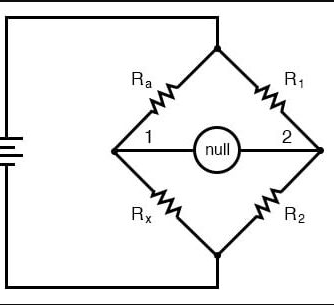
\includegraphics[width=0.4\linewidth]{media/puente-wheatstone}
	\caption{Esquema - Puente Wheatstone}
	\label{fig:puente-wheatstone}
\end{figure}

En la figura \ref{fig:puente-wheatstone} se puede apreciar el puente Wheatstone, estando equilibrado cuando los valore de resistencia $R1, R2, R_A y R_X$ sean igual en magnitud, obteniéndose solo valores aproximados para resistencias físicas, por lo que son requeridas resistencias de precisión para la medición de magnitudes de escala pequeña al hacer uso de sensores resistivos.

Por otro lado durante la experiencia se usaron resistencias de $1K \Omega$ con un variación porcentual del 5\% para la implementación del puente y haciendo uso un voltaje de DC de alimentación de 5V, obteniendo los voltajes común, diferencial entre los brazos los mostrados en la tabla \ref{tab:mediciones-DC-puente}.

\begin{table}[]
	\centering
	\begin{tabular}{|c|c|c|c|c|}
		\hline
		\textbf{Vin}                 & \textbf{V1}                 & \textbf{V2}                & \textbf{Vc}                 & \textbf{Vd}                   \\ \hline
		\multicolumn{1}{|r|}{5,0009} & \multicolumn{1}{r|}{2,4976} & \multicolumn{1}{r|}{2,505} & \multicolumn{1}{r|}{2,5013} & \multicolumn{1}{r|}{0,006352} \\ \hline
	\end{tabular}
	\caption{Mediciones DC - Puente Wheatstone}
	\label{tab:mediciones-DC-puente}
\end{table}

\section{Alimentación del puente con una fuente alterna}

Para este propósito durante la experiencia se hizo del generador de funciones configurar la amplitud de la señal de salida para la amplitud y frecuencia especificadas, sin embargo para la alimentación del circuito se uso un voltaje pico menor debido a que se considero una polarización a 5V para el amplificador de instrumentación, evitando de esta forma una saturación en la salida del circuito.

\begin{figure}[h]
	\centering
	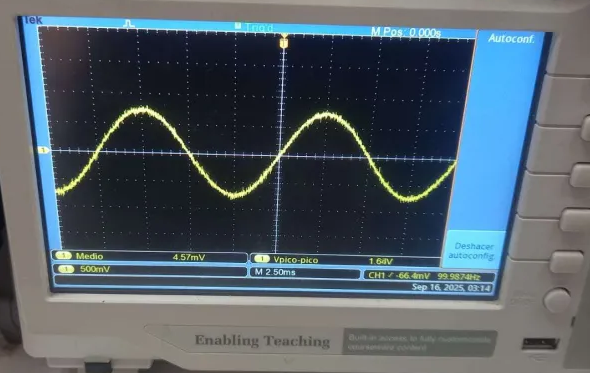
\includegraphics[width=0.4\linewidth]{media/senial-alterna}
	\caption{señal alterna de alimentación}
	\label{fig:senial-alterna}
\end{figure}

En la figura \ref{fig:senial-alterna} se puede apreciar la configuración para la señal de entrada a aplicar en los terminales de entrada del puente Wheatstone


\section{Ganancia en modo común AD620}

Para la obtención de una señal en modo común se hizo de los brazos del puente de resistencias, siendo en este caso el $V_1$ el que se uso como referencia para medir este medición el cual pertenece al lado izquierdo del puente como se muestre en la tabla \ref{tab:mediciones-DC-puente}, por otro lado en la parte del amplificador de instrumentación se tomaron los pines 2 y 3 (entradas inversora y no-inversora) como punto común de entrada para la salida de voltaje en $V_1$.

% TODO: \usepackage{graphicx} required
\begin{figure}[h]
	\centering
	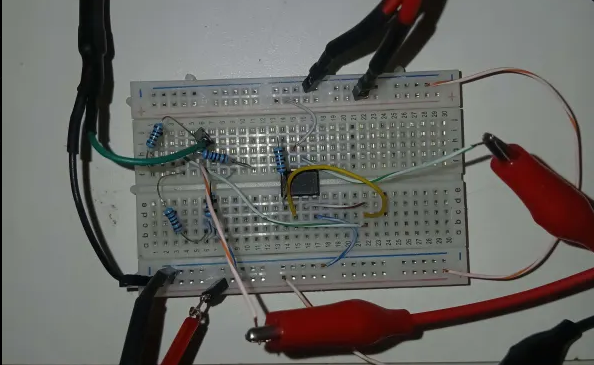
\includegraphics[width=0.5\linewidth]{media/implementacion}
	\caption{Implementación del puente de resistencias - Amplificador de instrumentación}
	\label{fig:implementacion}
\end{figure}

En la figura \ref{fig:implementacion} se muestra el circuito e implementación realizada, obteniendo finalmente un voltaje de salida y en modo común que se muestran en la tabla \ref{tab:mediciones-modo-comun}

\begin{table}[]
	\centering
	\begin{tabular}{|c|c|c|c|c|}
		\hline
		\textbf{Vin {[}Vp{]}} & \textbf{Vc {[}Vp{]}} & \textbf{Ac} & \textbf{Vc} & \textbf{Vd} \\ \hline
		0,26                  & 0,026                & 0,1         & 2,5013      & 0,006352    \\ \hline
	\end{tabular}
	\caption{Mediciones en modo común}
	\label{tab:mediciones-modo-comun}
\end{table}
































